\chapter{Introduction}
\label{chp:introduction}

Associative memories are believed to be one of the core mechanisms in human cognition: they allow us to classify sensory input in a fraction of a second and guide our thoughts along chains of semantic links \cite{palm2013neural}. The Willshaw associative memory model (also \acrlong{BiNAM}, \acrshort{BiNAM}) is one of the best understood, biologically plausible associative memory models \cite{steinbuch1961lernmatrix,BiNAM1969,palm1980associative}. In conjunction with the neuromorphic hardware systems developed as part of the \HBP \cite{hbp_projects}, an implementation of this model as spiking neural networks might provide a building block for the large-scale simulation of cognitive systems and serve as a benchmarking network which can be used to analyse the performance of said neuromorphic hardware. The goals of this thesis are to characterise the design space of a spiking Willshaw associative memory implementation and to develop measures and tools which can be used for both design space exploration and hardware benchmarking.

This chapter provides a high-level overview of this document: \cref{sec:motivation_goals} elaborates on the motivation and goals sketched in the previous paragraph, \cref{sec:structure} outlines the structure of the subsequent chapters and \cref{sec:notation} closes with some remarks on notational conventions.

\section{Motivation and goals}
\label{sec:motivation_goals}

Here, we draw a sketch of the topical framework that encompasses this thesis, and, in doing so, present and motivate the overall goals. The following sections can only give a rough overview. Mentioned topics are discussed in greater detail in the following chapters -- see the structure overview in \cref{sec:structure} for more information.

\subsection{Neuromorphic hardware systems in the Human Brain Project}

The \acrfull{HBP} is a European research project which aims at advancing the understanding of the structure and function of the human brain at multi-level scales. A key goal of the project is the development of neuromorphic hardware systems: special purpose computers designed to enable the simulation of large, brain-like circuits and to provide scientists with means to validate hypotheses regarding brain function \cite{hbp_objectives}.

In contrast to the firing-rate coded artificial neural networks, which today are ubiquitous in the field of machine learning, the \acrshort{HBP} neuromorphic platforms are based on spiking neural networks. Although still greatly simplified, spiking neural networks model processes in biological nervous systems more accurately than their firing-rate counterparts: neurons are represented as independent dynamic processes with asynchronous communication via electric pulses (spikes).

\begin{figure}
	\centering
	\subbottom[Spikey tabletop device]{
		\centering
		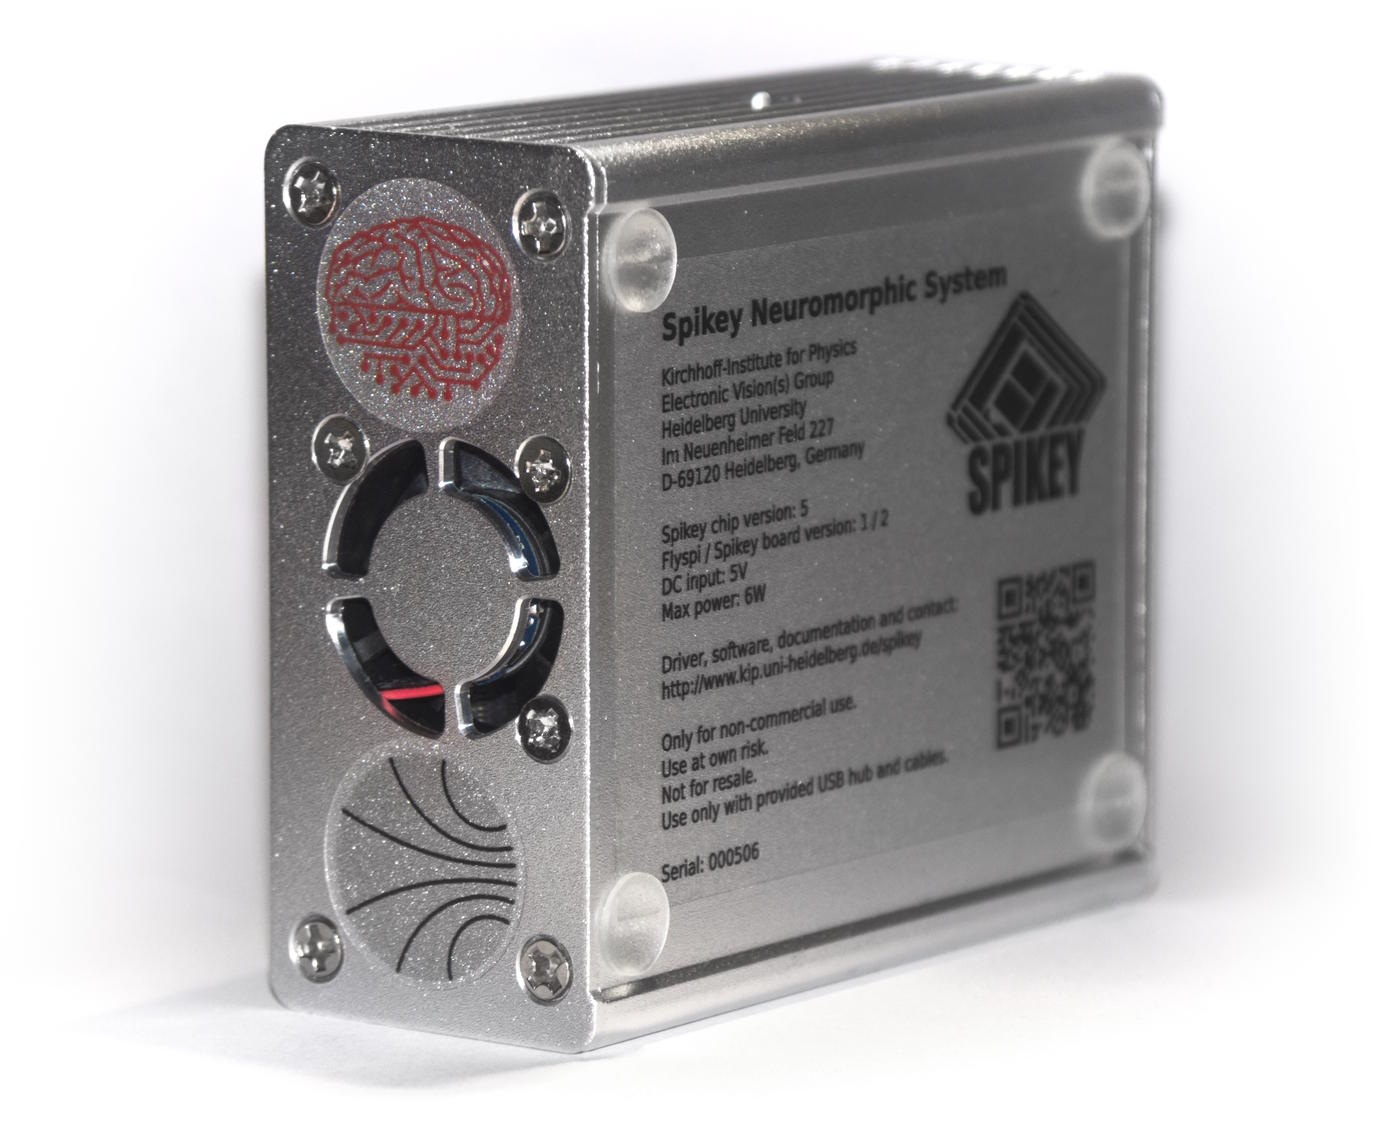
\includegraphics[width=0.475\textwidth]{media/chp1/spikey_photo.jpg}
		\label{fig:spikey_photo}
	}
	\subbottom[Spikey chip bonded to the circuit board]{
		\centering
		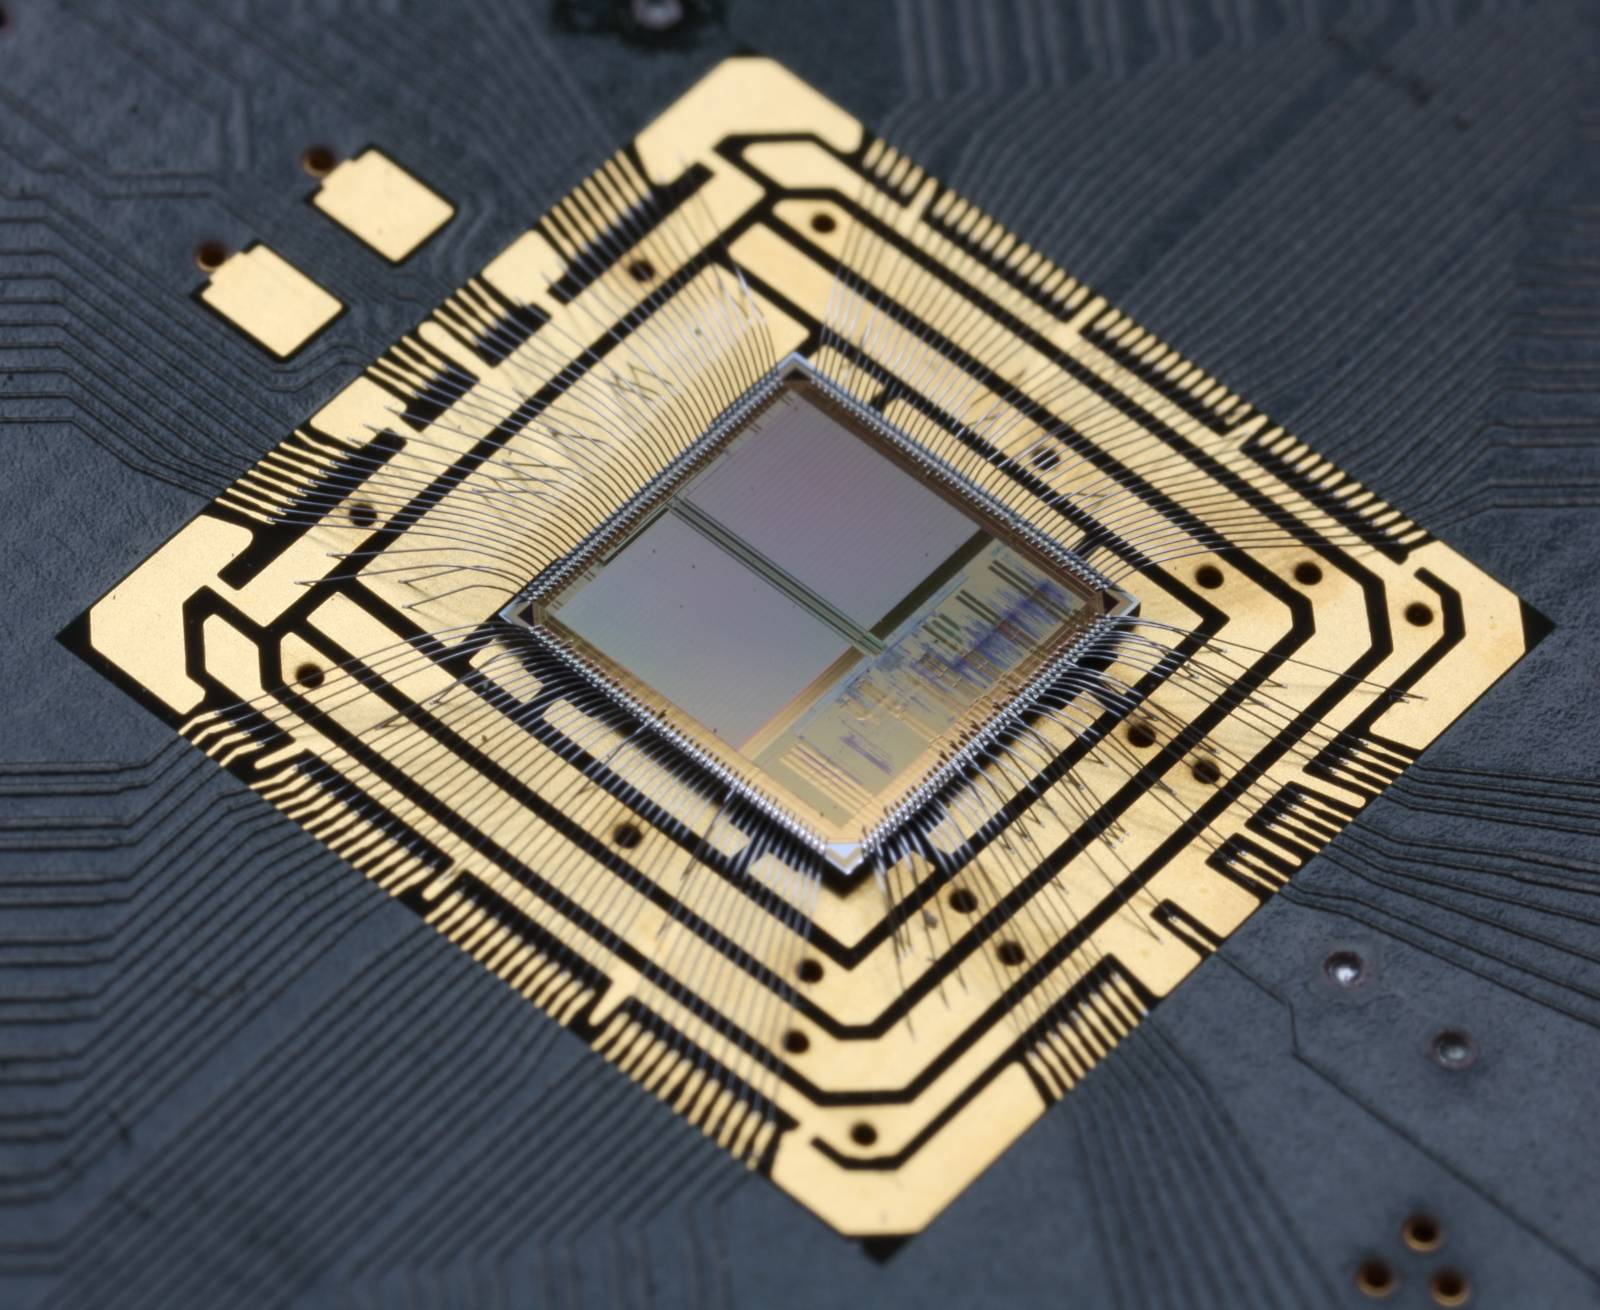
\includegraphics[width=0.475\textwidth]{media/chp1/spikey_chip_cropped.jpg}
		\label{fig:spikey_chip}
	}
	\caption[Photos of the Spikey neuromorphic hardware system]{Photos of the \emph{Spikey} neuromorphic hardware system developed by the Electronic Visions group at Heidelberg University. Size of the assembled device in (a) is about $8 \times 7 \times 3 \, \si{\centi\meter}$; the picture of the actual chip in (b) is copied from \url{http://www.kip.uni-heidelberg.de/spikey}.}
	\label{fig:spikey}
\end{figure}
\marginnote{A more technical description of the neuromorphic systems can be found in \cref{sec:neuromorphic_hardware}.}
The two neuromorphic hardware systems developed in the \acrshort{HBP} possess fundamentally different architectures. The \enquote{many-core system} \acrshort{NMMC} built at the University of Manchester is a fully digital computer, constructed around the \emph{SpiNNaker} chip \cite{furber2013overview}. In contrast, the \enquote{physical model} (\acrshort{NMPM}) built at Heidelberg University, is an analogue-digital mixed signal system composed of entire silicon wafers of \emph{HICANN} (\acrlong{HICANN}) chips \cite{schemmel2010wafer,bruderle2011comprehensive}. Both systems offer significantly faster simulation times for large spiking neural networks compared to software simulations on supercomputers, with \acrshort{NMMC} executing large networks at biological timescale and \acrshort{NMPM} with a speedup of $10\,000$ compared to biological timescale.

A third system -- which is used in addition to the already mentioned ones -- is the \emph{Spikey} neuromorphic system (\cref{fig:spikey}). The Spikey chip at its core is a predecessor of the HICANN in \acrshort{NMPM}. As such, it shares the same speedup factor of $10\,000$, but is limited to a single chip and features a less complex neuron model \cite{pfeil2013six}. Since Spikey has been in development for almost a decade now, both its hardware and software are in a relatively mature state.

\subsection{Willshaw associative memory as a spiking neural network}

\marginnote{Artificial neural networks in general and spiking neural networks in particular are discussed in \cref{sec:neural_network_models,sec:biophysical_neuron_model,sec:spiking_neuron_models}.}
Due to their time dynamic and asynchronous nature, spiking neural networks are difficult to design: every neuron possesses a multitude of parameters, and small changes in a single neuron parameter can dramatically influence the behaviour of the network as a whole. This is already true for the most simple class of network topologies, so called feed-forward networks, which do not allow recurrent connections (cycles in the network graph). On the other hand, it is reasonable to assume that biological neural networks have evolved with a robustness to neuronal variation. Indeed, the same neural circuits in two animals have been found to produce similar output on the network-level, although the intrinsic configuration of individual neurons varies significantly between the animals  \cite{prinz2004similar, marder2011multiple}.

\marginnote{The Willshaw associative memory model is described in detail in \cref{sec:willshaw_theory}.}
As the Willshaw associative memory model merely is a theoretical concept, that was not designed with the perils of dynamical systems in mind, it describes no mechanism that would allow for the compensation of neuronal imprecisions. On the contrary, each output signal is produced independently by a single artificial neuron. There is no possible way in which coarsely estimated neuron parameters could be absorbed by network-level effects. For the transition of the theoretical memory architecture to a spiking neural network we could proceed in two different ways. By designing robust sub-networks for each theoretical neuron from which the desired behaviour emerges, or by literally translating the theoretical model to a spiking neural network and tuning the neuron parameters to precise values.

We have decided to take the second approach. We aim at small and simple networks which only deviate slightly from the theoretical model, to ensure that the exhaustive theoretical results regarding the memory still apply. However, in order to find suitable neuron parameters, we need to provide an at least semi-automatic method which lets us choose \enquote{optimal} parameters for a given memory configuration.

\subsection{Associative memories as hardware benchmark}

The above decision on the spiking network architecture opens the door for another application. Since the network is scalable, possesses a highly regular and simple structure, and its theoretical behaviour under perfect conditions is well understood, it can serve as a hardware benchmark. Such a benchmark can be used to compare the performance of the individual platforms, and to quantify the influence of hard- and software changes.

Providing an assessable benchmarking network is important, as the \acrshort{HBP} hardware platforms (excluding Spikey) are currently in an early stage of development and running even simple networks reliably on all platforms is likely to be enough of a challenge. Ideally, sweeps along multiple parameter axes of the design space can be performed. This would allow to find regions for which the system shows abnormal behaviour. For example, varying the memory size might uncover scaling issues.

\subsection{Goals of this thesis}

The top-level goal of this thesis is to provide a working Willshaw associative memory (\acrshort{BiNAM}) implementation as spiking neural network which can be executed on the mentioned neuromorphic hardware systems. In order to fulfil this goal for varying memory configurations (\eg size, data properties), we need to find a way to explore the network design space. This requires that we have defined the design space itself and performance measures we can assign to every point in the space.

Unfortunately, and unsurprisingly, the design space is high-di\-men\-sion\-al, which prevents any exhaustive exploration. Therefore, we intend to develop and evaluate estimations of the network performance. These should allow an interactive exploration of a two-dimensional projection of the design space and help to restrict the parameter space to regions, in which time-consuming network simulations (potentially accelerated by the neuromorphic hardware) are sensible. Additionally, it should be possible to use the performance estimations for automatic parameter optimisation.

These goals also come with a significant engineering task, as the software tools for interactive design space exploration, parameter optimisation and execution on the hardware platforms have to be implemented. Finally, we have to investigate whether the built tools can be reliably used for benchmarking.

\section{Structure}
\label{sec:structure}

Whereas \cref{sec:motivation_goals} approached the topics in this thesis from a bird's-eye perspective and in no particular order, this section linearly trudges along the chapters and traces the golden thread which guides through the pages to come.

In \cref{chp:related_work}, we start by summarising the related work that sits at the foundation of this thesis: we touch the relevant neurobiological basics, introduce notable neuron and neural network models, and present the neuromorphic hardware platforms and software simulators. Finally, the Willshaw associative memory model (\acrshort{BiNAM}) is described and compared to other models.

In order to transition the theoretical \acrshort{BiNAM} model to a spiking neural network, \cref{chp:spinam} defines a parametrised set of spiking \acrshort{BiNAM} implementations. Combined with the neuron model parameters, these implementation parameters span the associative memory design space we seek to explore. Various associative memory evaluation measures are then proposed, which allow the assignment of a set of scores to any given point in the design space. As a side-effect, these measures allow comparison -- and eventually benchmarking -- of different hardware and software platforms. The chapter concludes with thoughts on \acrshort{BiNAM} test data generation. In its entirety, the material in \cref{chp:related_work,chp:spinam} allows the construction of a complete \acrshort{BiNAM} design space exploration pipeline.

Armed solely with the methods described beforehand, however, any even rudimentarily exhaustive design space exploration would be infeasible, regardless of neuromorphic hardware acceleration. Thus, \cref{chp:neuron_evaluation} takes a step back and describes \acrshort{BiNAM} performance estimates of varying complexity, based on single neuron simulation. To achieve the fastest possible execution speed, we compare the performance of various numerical differential equation integration methods. Finally, a method for fractional neuron output spike count estimation is presented, which in conjunction with a naive Downhill-Simplex algorithm effectively allows automated neuron parameter optimisation with respect to a given set of network parameters. The presented work can be used to limit the parameter space to interesting regions, which can then be explored by means of expensive full network simulations.

Such simulations are conducted in \cref{chp:experiments}, which describes experiments testing the evaluation measures defined in \cref{chp:spinam} on the neuromorphic hardware platforms. The hardware results are then compared to software simulations and the coarse estimates from the fourth chapter.

Finally, \cref{chp:conclusion} summarises the insights obtained and lists possible future work that was out of scope for this thesis.

\section{Notational conventions}
\label{sec:notation}

\marginnote{Margin notes contain additional remarks or small sketches which aim at providing a better understanding of the material -- however, they can be safely skipped; all relevant information is presented in the main text.}
This section informally lists some important notational conventions employed throughout the thesis.

\paragraph{Symbols}
Great care has been taken to consistently impose a single meaning on most mathematical symbols. Exceptions to this rule are \enquote{local variables}, including -- but not limited to -- the symbols $i, j, k, \ell$ which are used as generic indices, for example as summation indices, loop counters or to point at a generic element of a set, tuple, vector or matrix. The meaning of symbols used in more than one occasion can be looked up in the symbol overview in the appendix.

\paragraph{Vector and matrix indices}
Vectors are marked as such with a vector arrow and are generally assumed to be column vectors. If individual matrix or vector elements are accessed, this is denoted as $(\vec x)_i$ (the $i$-th component of $\vec x$) or $(M)_{ij}$ (the element in the $i$-th row and $j$-th column of the matrix $M$) respectively. An exception to this rule are algorithms in pseudo-code where individual vector and matrix elements are accessed in the \enquote{square brackets}-notation, for example $\vec x[i]$ and $M[i, j]$. Regardless of the notation, vector and matrix indices follow the mathematical convention and always start with one.

\paragraph{Sets and tuples}
Sets are usually typeset in fraktur (\eg $\mathfrak{b}$, $\mathfrak{B}$). Double-struck letters (\eg $\B, \N, \R$) denote ranges of numbers. The operator \enquote{$\Arrowvert$} denotes the concatenation of two tuples: let $a = (a_1, \ldots, a_i)$ and $b = (b_1, \ldots, b_j)$ denote two sequences of length $|a| = i$ and $|b| = j$. The operation $a \Arrowvert b$ is then defined as:
\begin{align}
	a \Arrowvert b = (a_1, \ldots, a_i, b_1, \ldots, b_j)
\end{align}

\paragraph{Discontinuities in differential equations}
Spiking neural network models are generally formulated as differential equations. However, they contain discontinuities which often are expressed in the literature with the help of the Dirac delta $\delta(t)$:
\begin{align}
 	\int_{-\infty}^{\infty} f(t) \cdot \delta(t) \; \mathrm{d}t = f(0) \,.
\end{align}
Use of the Dirac delta may facilitate mathematical analysis, but in the opinion of the author tends to obscure the actual concept that is being described. We therefore use a less mathematical notation which involves the \enquote{$\gets$} (read \enquote{gets}) operator. For example, a differential equation with a discontinuity at time $t_0$ is described as
\begin{align}
	\dot u(t) &= g \cdot (u(t) - u_0) \,,\\
	u(t) &\gets u(t) + \Delta u \quad \text{if } t = t_0\,,
\end{align}
and supposed to be equivalent to the more \enquote{correct} mathematical notation
\begin{align}
	\dot u(t) = g \cdot (u_0 - u(t)) + \delta(t - t_0) \cdot \Delta u\,.
\end{align}
